\documentclass[14pt]{beamer} %Makes presentation
%\documentclass[handout]{beamer} %Makes Handouts
\usetheme{Singapore} %Gray with fade at top
\useoutertheme[subsection=false]{miniframes} %Supppress subsection in header
\useinnertheme{rectangles} %Itemize/Enumerate boxes
\usecolortheme{seagull} %Color theme
\usecolortheme{rose} %Inner color theme

\definecolor{light-gray}{gray}{0.75}
\definecolor{dark-gray}{gray}{0.55}
\setbeamercolor{item}{fg=white}
\setbeamercolor{enumerate item}{fg=dark-gray}

\setbeamertemplate{navigation symbols}{}
%\setbeamertemplate{mini frames}[default]
%\setbeamercovered{dynamics}
\setbeamerfont*{title}{size=\large,series=\bfseries}
\setbeamerfont{footnote}{size=\tiny}

%\setbeameroption{notes on second screen} %Dual-Screen Notes
%\setbeameroption{show only notes} %Notes Output

\setbeamertemplate{frametitle}{\vspace{.5em}\bfseries\insertframetitle}
\newcommand{\heading}[1]{\noindent \textbf{#1}\\ \vspace{1em}}

\usepackage{bbding,color,multirow,times,ccaption,tabularx,graphicx,verbatim,booktabs}
\usepackage{amsmath}
\usepackage{colortbl} %Table overlays
\usepackage[english]{babel}
\usepackage[latin1]{inputenc}
\usepackage[T1]{fontenc}
\usepackage{lmodern}

%\author[]{Thomas J. Leeper}
\institute[]{
  \inst{}%
  Department of Government\\London School of Economics and Political Science
}

\usepackage{tikz}
\usetikzlibrary{shapes,arrows}

\title{Welcome and First Lecture}

\date[]{}

\begin{document}

\frame{\titlepage}

\frame{\tableofcontents}

\section{Background/Context}
\frame{\tableofcontents[currentsection]}

\frame{

\frametitle{Experiments}

Oxford English Dictionary defines ``experiment'' as:

\begin{enumerate}
\item A scientific procedure undertaken to make a discovery, test a hypothesis, or demonstrate a known fact
\item A course of action tentatively adopted without being sure of the outcome
\end{enumerate}
}

\frame{

\frametitle{Experiments}

\begin{itemize}\itemsep0.75em
\item ``Experiments'' have a very long history

\item Major advances in design and analysis of experiments based on agricultural and later biostatistical research in the 19th century
	\begin{itemize}
	\item R.A. Fisher
	\item Jerzy Neyman
	\item Karl Pearson
	\item Oscar Kempthorne
	\end{itemize}

\end{itemize}

}

\frame{

\frametitle{In Social Sciences}

\small

\begin{itemize}
\item ``Experiments'' emerged in psychology 19th century
	\begin{itemize}\footnotesize
	\item Not randomized -- more like ``What if?'' studies
	\item Heavily laboratory-based or clinical
	\end{itemize}
\item<2-> First randomized, controlled trial (RCT) by Peirce and Jastrow in 1884
\item<3-> RCTs came later to medicine (circa 1950)
\item<4-> And have been a major part of the ``credibility revolution'' in economics
	\begin{itemize}
	\item See, especially, LaLonde (1986)
	\end{itemize}
\end{itemize}

}


\frame{

\frametitle{In Social Science I}

\begin{itemize}\itemsep0.5em
\item APSA Pres. A. Lawrence Lowell (1922):\\
{\small
\textit{``We are limited by the impossibility of experiment. Politics is an observational, not an experimental science\dots''}
}
\item<2-> First experiment by Gosnell (1924)
\item<3-> Gerber and Green (2000) first major experiment in political science
\end{itemize}

}

\frame{

\frametitle{{\large In Social Science II}}

\small

\begin{itemize}
\item Rise of surveys in the behavioral revolution
\item Survey research was not experimental because interviewing was still mostly paper-based
	\begin{itemize}
	\item ``Split Ballots'' (Schuman \& Presser; Bishop)
	\end{itemize}
\item<2-> 1983: Merrill Shanks and the Berkeley Survey Research Center develop CATI
\item<3-> Mid-1980s: Paul Sniderman \& Tom Piazza performed the first survey experiment\only<3->{\footnote{Sniderman, Paul M., and Thomas Piazza. 1993. \textit{The Scar of Race}. Cambridge, MA: Harvard University Press.}}
	\begin{itemize}\footnotesize
	\item Then: the ``first multi-investigator''
	\item Later: Skip Lupia and Diana Mutz created TESS
	\end{itemize}

\end{itemize}

}


\frame{

\frametitle{{\large In Social Science III}}

\small

\begin{itemize}\itemsep1em
\item Field experiments emerge in the 1990s
	\begin{itemize}
	\item Voter mobilization
	\item Poverty alleviation
	\end{itemize}

\item The ``credibility revolution'' in economics in the 2000s
	\begin{itemize}
	\item Rise in academic and public/private-sector use of RCTs
	\item Diversification of topical focus: political conflict/violence, legislative representation, tax policy
	\end{itemize}
	
\item Mid-2010's see emergence of experiment-driven ``behavioural science'' and ``behavioural public policy''
	\begin{itemize}
	\item We now live in the ``nudge'' era
	\end{itemize}
\end{itemize}

}


\frame{
\frametitle{Evidence-based Policy}

\begin{itemize}\itemsep1em
\item Experiments have been a focal part of ``evidence-based policymaking''
	\begin{itemize}
	\item Evidence-based medicine
	\item Evidence-based education
	\item Evidence-based budgeting
	\item Evidence-based politics?
	\end{itemize}
	
\item<2-> In the US, UK, and elsewhere politicians and bureaucrats face pressure to know ``what works?'' and to implement policies that ``work''

\item<3-> Experiments are seen as a particularly useful --- but perhaps limited --- way to know ``what works''
\end{itemize}

}


\frame{

\frametitle{Experiments Raise Big Questions}

\begin{enumerate}\itemsep1em
\item<2-> What can we learn from experiments? What \textit{can't} we learn from experiments?

\item<3-> Are experiments always a credible research method? When can experiments fail?

\item<4-> Can we generalize from experiments to the ``real world''?

\item<5-> When is it ethically acceptable to experiment on people?

\end{enumerate}

}

\frame{\huge\vskip20pt\textbf{Questions?}}

\frame{}



\section{Experimental Primer}
\frame{\tableofcontents[currentsection]}

\frame{

\frametitle{{\normalsize What kinds of questions can we answer with experiments?}}

\normalsize

\begin{itemize}\itemsep1em
\item<2-> Forward causal questions
	\begin{itemize}
	\item Can X cause Y?
	\item What effects does X have?
	\end{itemize}
\item<3-> Backward causal questions
	\begin{itemize}
	\item What causes Y?
	\item How much of Y is attributable to X?
	\end{itemize}
\end{itemize}
}



\frame{

\frametitle{Principles of causality}

\begin{enumerate}\itemsep1em
\item \textbf<2->{Correlation/Relationship}
\item \textbf<2->{Nonconfounding}
\item \textbf<2->{Direction (``temporal precedence'')}

\vspace{1em}

\item Mechanism

\vspace{0.5em}

\item Appropriate level of analysis
\end{enumerate}
}


% Causal graphs
\begin{frame}
\begin{center}
\begin{tikzpicture}[>=latex',circ/.style={draw, shape=circle, node distance=5cm, line width=1.5pt}]
    \draw (0,0) node[left] (X) {\textcolor<2->{red}{Smoking}};
    \draw[->] (X) -- (5,0) node[right] (Y) {Cancer};
    \draw[->] (-3,3) node[above] (Z) {Sex} -- (X);
    \draw[->] (Z) -- (Y);
    \draw[->] (5,2) node[above] (A) {Environment} -- (Y);
    \draw[->] (4,-3) node[below, text width=3cm, align=center] (E) {Genetic\\Predisposition} -- (Y);
    \draw[->] (-2, -2) node[below, text width=2.5cm, align=center] (W) {Parental\\Smoking} -- (X);
    \draw[->] (W) -- (Y);
    \draw<2->[->, dashed, very thick] (E) -- (X);
\end{tikzpicture}
\end{center}
\end{frame}

\frame{

\frametitle{Establishing Relationship}

\begin{itemize}\itemsep1em
\item This is fairly trivial
\item Simply find value of $Corr(X,Y)$
\item In causal inference we often talk about correlations in terms of \textit{differences}
	\begin{itemize}
	\item Difference in values of $Y$ across values of $X$
	\item The presence of a difference indicates a correlation
	\end{itemize}
\end{itemize}

}

\frame{

\frametitle{Addressing Confounding}

In observational studies, we address confounding by:

\begin{enumerate}\itemsep1em
\item<2-> Correlating a ``putative'' cause ($X$) and an outcome ($Y$)
\item<3-> Identifying all possible confounds (\textbf{Z})
\item<4-> ``Conditioning'' on all confounds
	\begin{itemize}
	\item Calculating correlation between $X$ and $Y$ at each combination of levels of \textbf{Z}
	\end{itemize}
\end{enumerate}

}

\frame{

\frametitle{Temporal Precedence}

\begin{itemize}\itemsep0.5em
\item Even if an observational design identifies a relationship and credibly addresses sources of confounding, it still may not be a credible causal inference

\item<2-> ``Reverse causality'' is vague, referring to:
	\begin{itemize}
	\item Ambiguity about causal ordering, or
	\item Sequentially reinforcing causality between $X$ and $Y$
	\end{itemize}

\item<3-> Causation is strictly forward moving in time

\item<4-> $X$ must precede $Y$ in time for $X$ to cause $Y$

	\begin{itemize}
	\item $X$ can be \textit{measured} after $Y$ as long as it comes before it
	\end{itemize}
	
\end{itemize}

}


\frame{

\frametitle{Experiments are different}

\begin{enumerate}\itemsep0.75em
\item<2-> Draw causal inferences through \textit{design} not \textit{analysis}
\item<3-> Randomization breaks selection bias
\item<4-> We don't need to ``control'' for anything
\item<5-> We see ``causal effects'' in the comparison of experimental groups
\end{enumerate}

}


\begin{frame}
\small 
\begin{center}
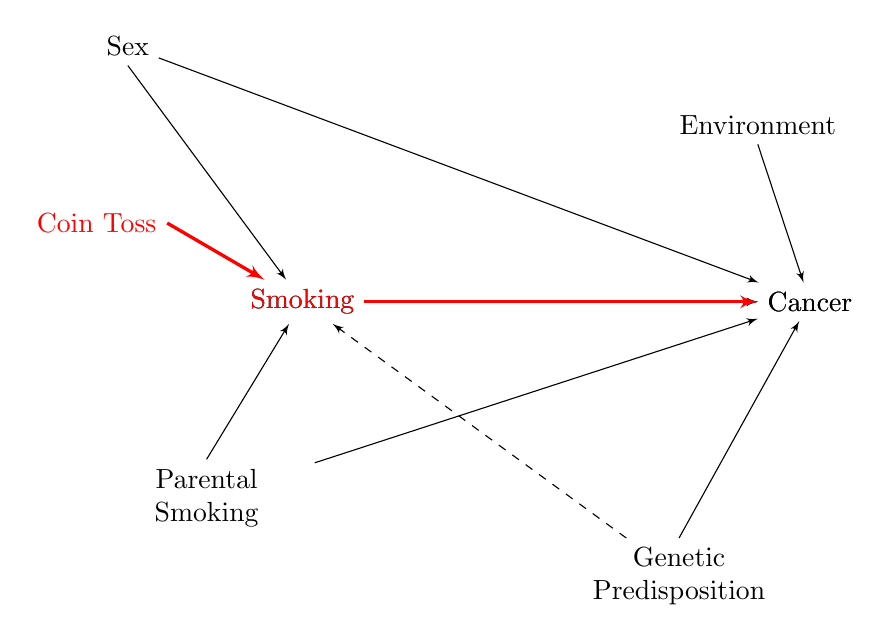
\begin{tikzpicture}[>=latex',circ/.style={draw, shape=circle, node distance=5cm, line width=1.5pt}]
    \draw<1>[->] (0,0) node[left] (X) {Smoking} -- (5,0) node[right] (Y) {Cancer};
    \draw<2>[->] (0,0) node[left, color=red] (X) {Smoking} -- (5,0) node[right] (Y) {Cancer};
    \draw[->] (-3,3) node[above] (Z) {Sex} -- (X);
    \draw[->] (Z) -- (Y);
    \draw[->] (5,2) node[above] (A) {Environment} -- (Y);
    \draw[->] (4,-3) node[below, text width=3cm, align=center] (E) {Genetic\\Predisposition} -- (Y);
    \draw[->] (-2, -2) node[below, text width=2.5cm, align=center] (W) {Parental\\Smoking} -- (X);
    \draw[->] (W) -- (Y);
    \draw[->, dashed] (E) -- (X);
    
    \draw<2->[->, very thick, color=red] (-2.5,1) node[left, color=red] (Tr) {Coin Toss} -- (X);
    \draw<2->[->, very thick, color=red] (X) -- (Y);
\end{tikzpicture}
\end{center}
\end{frame}




% Mill's method of difference
\frame{
\frametitle{{\normalsize Mill's Method of Difference}}

\small

If an instance in which the phenomenon under investigation occurs, and an instance in which it does not occur, \textbf<2->{have every circumstance save one in common}, that one occurring only in the former; \textbf<2->{the circumstance in which alone the two instances differ, is the} effect, or \textbf<2->{cause}, or an necessary part of the cause, \textbf<2->{of the phenomenon}.
}


\frame{

\frametitle{Definitions}

\begin{itemize}\itemsep0.75em
\item<2-> A randomized experiment, or randomized control trial (RCT) is:
\end{itemize}
	\begin{quote}\small
		The observation of units after, and possibly before, a randomly assigned intervention in a controlled setting, which tests one or more precise causal expectations
	\end{quote}
\begin{itemize}\itemsep0.75em
\item<3-> If we manipulate the thing we want to know the effect of ($X$), and control (i.e., hold constant) everything we do not want to know the effect of ($Z$), the only thing that can affect the outcome ($Y$) is $X$.
\end{itemize}

}


\frame{\huge\vskip20pt\textbf{Questions?}}






\section{Introductions}
\frame{\tableofcontents[currentsection]}

\frame{
\frametitle{Who am I?}

\small

\begin{itemize}\itemsep0.25em

\item Thomas Leeper

\item Assistant Professor in Political Behaviour

\item Originally from Minnesota (USA)

\item Interested in public opinion and political psychology

\item Office hours:\\
Mon 10:30--1:30; Fri 9:30-10:30 CON 4.11\\
(Sign-up on LSE for You)\\
Otherwise, email: \href{mailto:T.Leeper@lse.ac.uk}{T.Leeper@lse.ac.uk}

\end{itemize}

}


\frame{

\frametitle{Who are you?}

\begin{itemize}\itemsep1em

\item Where are you from?

\item What interests you about government or politics?

\item What do you hope to learn from the course?

\end{itemize}

}



\section{Administrative Stuff}
\frame{\tableofcontents[currentsection]}

\frame{

\frametitle{Course Resources}

\small

\begin{itemize}\itemsep0.25em
\item Reading List:\\
\url{https://lse.rl.talis.com/lists/BA9D65E3-F764-8018-1883-4587DCB78F4F.html}

\item Gelnnerster and Takavarasha's \textit{Running Randomized Evaluations}

\item Moodle:\\
\url{https://moodle.lse.ac.uk/course/view.php?id=5709}
	\begin{itemize}
	\item Slides (after lecture)
	\item Forums
	\item Assignments
	\end{itemize}
\end{itemize}
}

\frame{

\frametitle{Textbook}

\begin{center}
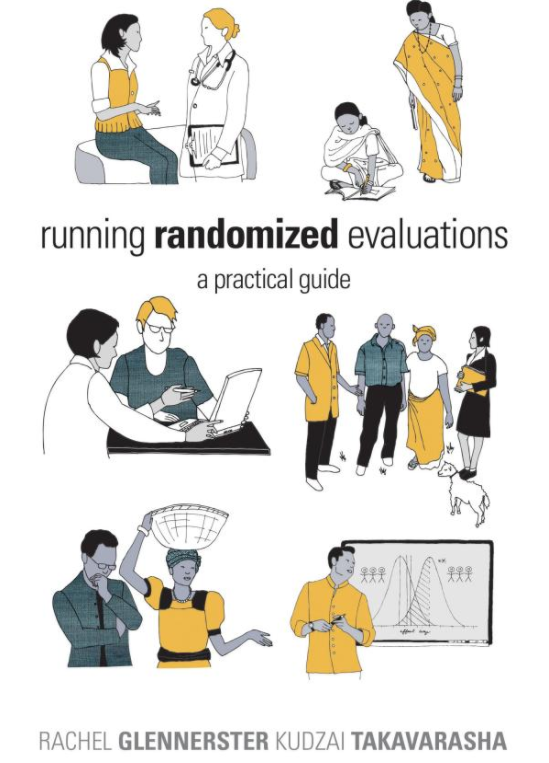
\includegraphics[height=0.75\textheight]{images/rre}
\end{center}

}



\frame{

\frametitle{{\large Schedule: Michaelmas Term}}

\footnotesize

MT 1 Introduction (Sep. 29) \\
MT 2 Statistical Foundations I (Oct. 6) \\
MT 3 Statistical Foundations II (Oct. 13) \\
MT 4 Practical Issues (Oct. 20) \\
MT 5 The Politics of Evidence (Oct. 27) \\
\textit{Reading Week} \\
MT 7 Substantive Topic 1 (Nov. 10) \\
MT 8 Substantive Topic 2 (Nov. 17) \\
MT 9 Substantive Topic 3 (Nov. 24) \\
MT 10 Substantive Topic 4 (Dec. 1) \\
MT 11 Substantive Topic 5 and Conclusion (Dec. 8) \\
ST 1 Revision Session (Apr. 27) \\

}


\frame{

\frametitle{Substantive Topics?}

This is your decision! What should we discuss?

{\footnotesize

\begin{itemize}
\item Voter mobilization
\item Social media
\item Poverty alleviation
\item Political development
\item Policy nudges
\item Political representation
\item Public health
\item \dots
\end{itemize}
}

Decide over next 2--3 weeks!

}

\frame{

\frametitle{Learning Outcomes}

\small

\begin{enumerate}\itemsep0.25em
\item Describe the logic of randomized experimentation for studying causal effects of interventions in comparison to other approaches.
\item Evaluate the strengths, weaknesses, and ethics of experiments as a research design and evaluation method.
\item Analyse the use and utility of experimental methods in real-world cases.
\item Apply the logic of experimental methods to political science research questions.
\end{enumerate}

}

\frame{

\frametitle{Summative Assessment}

\begin{itemize}\itemsep1em
\item Breadth: 90-minute written exam (ST)

\item Depth: 2,250-word summative essay consisting of either:
	
	\begin{enumerate}
	\item Research Proposal, or
	\item Journalistic Case Study
	\end{enumerate}

\item Deadline for essay is \textbf{5 December 2017}

\item Exam and essay each count equally (50\%)
\end{itemize}

}

\frame{

\frametitle{Summative Essay: Option A}

Craft an experimental research design:

\begin{itemize}\itemsep0.5em

\item Research question
\item Theoretical contribution
\item Testable hypotheses
\item Description of the proposed data collection and analysis

\end{itemize}

}

\frame{

\frametitle{Summative Essay: Option B}

Write a case study of ``real-world'' use of experimentation:

\begin{itemize}\itemsep0.5em

\item Identify a recent use of experimentation in a public or private sector setting
\item Describe the experiment(s) and what was learned
\item Critically evaluate how the experiment(s) informed policy, debate, or practice

\end{itemize}

}


\frame{

\frametitle{Formative Assessment}

\begin{enumerate}\itemsep2em
\item Presentation of final essay topics in Weeks 9 and 10

\item Technical problem set due in MT Week 5
\end{enumerate}

}




\frame{\huge\vskip20pt\textbf{Questions?}}


\appendix
\frame{}

\end{document}
